\documentclass[a4paper]{article}
\usepackage[pdftex]{graphicx}
\usepackage[utf8]{inputenc}
\usepackage{enumerate}
\usepackage{icomma}
\usepackage{siunitx}
\sisetup{locale=DE} 
\usepackage{amssymb}
\usepackage{tikz}
\usepackage{href-ul}
\hypersetup{
	colorlinks=true,
	linkcolor=blue,
	urlcolor=blue}
\usepackage{geometry}
\geometry{a4paper, top=15mm, left=15mm, right=15mm, bottom=15mm,
	headsep=10mm, footskip=12mm}

\begin{document}
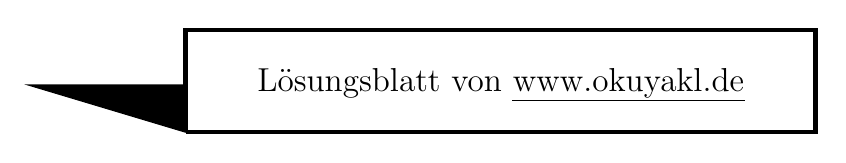
\begin{tikzpicture}(10,3)
	\draw[ultra thick](2,0) --(10,0) -- (10,1.3) --(2,1.3) -- (2,0);
	\draw[fill=black](2,0)-- (0,.6) -- (2,.6) -- (2,0);
	\node at (6,.6) {\large Lösungsblatt von \href{https://www.okuyakl.de}{www.okuyakl.de}};
\end{tikzpicture}
\vspace{0.5 cm}


\noindent{\bf Aufgabe 1.}\\
Die blaue Fläche besteht aus zwei Kreissegmenten mit dem Radius $a$ und dem Mittelpunktswinkel $\mu = 90^\circ$ ({\it Ein Kreissegment berechnet sich mit der Fläche eines Kreissektors minus der Fläche des Dreiecks}):
$$ A_{blau}= 2 \cdot \left( {90^\circ \over 360^\circ} \cdot \pi \cdot a^2 - {1 \over 2}a^2 \right) =
\left( {\pi \over 2} - 1 \right) \cdot a^2  $$
\noindent{\bf Aufgabe 1. b)}\\
Die schraffierte Fläche ist ebenfalls ein Kreissegment mit dem Mittelpunktswinkel 
$\mu=90^\circ$, aber mit dem Radius 
$$r_s=\sqrt{a^2+a^2} = \sqrt{2} \cdot a$$
Die Dreiecksfläche ist $a^2$. 
$$A_{sch}= {90^\circ \over 360^\circ} \cdot \pi \cdot (\sqrt{2}a)^2 - a^2= 
{\pi \over 4} \cdot 2a^2- a^2 = \left({\pi \over 2} -1\right) \cdot a^2 = A_{blau}$$

\noindent {\bf Aufgabe 2.}\\
Die Fläche des Kreissektors ist:
$$A_{KS}={\mu \over 360^\circ} \cdot \pi \cdot r^2 = {70^\circ \over 360^\circ}\cdot \pi \cdot ( \SI{4}{\centi\meter})^2=\underline{\SI{9,77}{\centi\meter^2}}$$
Die Fläche des Dreiecks $ABM$ ist:
$$A_{\Delta}={1\over 2}r^2 \cdot \sin{\mu}={1\over 2}(\SI{4}{\centi\meter})^2 \cdot \sin{70^\circ}=\underline{\SI{7,52}{\centi\meter^2}}$$
Die Fläche des Kreissektors ist, bezogen auf die Fläche des Dreiecks, um diesen Prozentsatz größer:
$$p={A_{KS} - A_{\Delta}\over A_{\Delta}}\cdot 100\% =\underline{30\%}$$

\noindent
\fbox{
	\begin{minipage}{0.47\textwidth}
	\noindent {\bf Aufgabe 3.}\\
	Der Umfang besteht aus zwei Kreisbögen plus der Radiuslänge.
	$$
	\renewcommand{\arraystretch}{2}
	\begin{array}{rcl}
	U &=& 2 \cdot b + r \\
	&=& 2 \cdot {60^\circ \over 180^\circ}\cdot \pi \cdot 1,5 +1,5 \\
	&=& 4,64~m
	\end{array}
	$$
	Die Fläche setzt sich zusammen aus zwei Kreissektoren, von denen ein gleichseitiges Dreieck abzuziehen ist.
	$$
	\renewcommand{\arraystretch}{2}
	\begin{array}{rcl}
	A &=& 2 \cdot A_{SEK} - A_\Delta \\
	&=& 2 \cdot {60^\circ \over 360^\circ} \cdot  \pi 1,5^2 - {1\over 2} \cdot 1,5^2 \cdot \sin 60^\circ\\
	&=& 1,38~m^2 
	\end{array}
	$$	
	\end{minipage}
}
\noindent
\fbox{
	\begin{minipage}{0.47\textwidth}
	\noindent {\bf Aufgabe 4.}\\
	Die Fläche setzt sich zusammen aus einem gleichseitigem Dreieck der Länge $2r$ minus drei  sechstel Kreisen, also einem Halbkreis mit Radius $r$.
	$$
	\renewcommand{\arraystretch}{2}
	\begin{array}{rcl}
	A &=& A_\Delta - A_{HK}\\
	&=& {1 \over 2} \cdot (2r)^2 \cdot \sin(60^\circ)-{1\over 2} \pi r^2 \\
	&=& (\sqrt{3} - {1 \over 2}\pi)~r^2 \\
	&=& 0,16 \cdot r^2
	\end{array}
	$$ 	
	\end{minipage}
}
\vspace{0.5 cm}


\noindent {\bf Aufgabe 5.}\\
Wir rechnen: Fläche = Großer Kreissektor minus Halbkreis plus kleines Kreissegment.\\
Kleines Kreissegment = Kleiner Kreissektor minus kleines gleichseitiges Dreieck.
$$
\renewcommand{\arraystretch}{2}
\begin{array}{rcl}
A &=& A_{SEK}-A_{HK}+(A_{sek}-A_\Delta)= A_{SEK}-A_{HK}+A_{sek}-A_\Delta\\
 &=& {60^\circ \over 360^\circ}\cdot \pi (2r)^2-{1\over 2}\pi r^2 + {60^\circ \over 360^\circ}\cdot \pi r^2- {1 \over 2} \cdot r^2 \cdot \sin(60^\circ)\\
 &=& ({2\over 3}\pi - {1\over 2}\pi +{1\over 6} \pi -{1 \over 4}\sqrt{3})~r^2=  ({1\over 3} \pi - {1 \over 4}\sqrt{3})~r^2\\
 &=& 0,614~r^2
\end{array}
$$

\newpage
\noindent{\bf Aufgabe 6. a)}\\
In die Figur können zwei gleichseitige Dreiecke mit der Seitenlänge $a$ einbeschrieben werden. Die äußere Linsenform besteht aus zwei Kreissegmenten mit dem Radius $a$ und dem Mittelpunktswinkel $\mu=120^\circ$ .
Ein solches Kreissegment hat den Flächeninhalt:
$$A_1={\mu \over 360^\circ}\cdot \pi a^2 - {1\over 2} a^2 \cdot \sin{\mu}={\pi \over 3} a^2-{\sqrt{3}\over 4} a^2$$
Die Iris ist ein Kreis mit dem Radius $a/2$. Ihre Fläche ist:
$$A_2=\pi \cdot \left({a \over 2}\right)^2 = {\pi \over 4} a^2$$
Die Pupille setzt sich zusammen aus zwei Kreissegmenten mit dem Radius $a$ und dem Mittelpunktswinkel $\mu=60^\circ$:
$$A_3={\mu \over 360^\circ}\cdot \pi a^2 - {1\over 2} a^2 \cdot \sin{\mu}={\pi \over 6} a^2-{\sqrt{3}\over 4} a^2$$
Die gesamte blaue Fläche setzt sich zusammen aus:
$$
\renewcommand{\arraystretch}{2}
\begin{array}{rcl}
A_{ges} &=& 2\cdot A_1 - A_2 + 2 \cdot A_3\\
A_{ges} &=& 2(\cdot {\pi \over 3} a^2-{\sqrt{3}\over 4}a^2) -  {\pi \over 4} a^2 + 2({\pi \over 6} a^2-{\sqrt{3}\over 4} a^2 )\\
A_{ges} &=& a^2 \cdot ( {2 \pi \over 3} -{\sqrt{3}\over 2}- {\pi \over 4}+{\pi \over 3}-{\sqrt{3}\over 2})\\
A_{ges} &=& a^2 \cdot ({3 \pi \over 4}-\sqrt{3})\quad (*)
\end{array}
$$

\noindent{\bf Aufgabe 6. b)}\\
Wir setzen $a=\SI{8}{\centi\meter}$ in $(*)$ ein und erhalten:
$$A_{ges}= (\SI{8}{\centi\meter})^2 \cdot ({3 \pi \over 4}-\sqrt{3})= \SI{64}{\centi\meter^2}\cdot 0,624 = \SI{39,9}{\centi\meter^2}$$

\begin{center}
	\includegraphics[width=7 cm]{../../viecher/endcomic.pdf}
	
	Hier geht es zurück zum \href{https://www.okuyakl.de/math/m10kreibL027/aa027.pdf}{Aufgabenblatt}
\end{center}

\end{document}

